\section{Method}
\subsection{Game Mechanics in Simulations}
Originally, we have considered simplifying the game mechanics by having a specific starting state and have a very fixed way of spawning new tiles to reduce randomness. However, we believe that this will defeat the whole point of the game, which mainly involves making moves that will limit the damage of randomness could do to our game. Thus, we have decided to follow the exact game mechanics with no reduction and simplification in the rules. This means that we will always start with a random board with 2 tiles with values on each of the tiles "2" or "4". Then, after each valid move, a new tile with values "2" or "4" will be generated  on a random empty tile. We loose when no valid moves are allowed.

\subsection{Representation and Q-value Calculation}
In our experiment, we have tried 2 types of representation, which are the simple representation and the relationship representation. They will be explained as follows. To calculate the q-value, we will use the linear approximation approach for simplicity.

\subsubsection{Simple Representation}
This is the simplest type of representation of our game, which is just simply a vector of 16 elements with each element representing the values of the individual tiles. For example, if we look at figure \ref{fig:game_board}, the state will simply be:
\begin{equation*}
\phi = (0,0,2,4,0,0,4,8,0,2,16,32,0,2,2,16)^{T}
\end{equation*}
To calculate the q-value, we will use our state vector acting on the weight vector representing each action, which can be written as:
\begin{equation*}
q_{a} = \phi ^{T} w_{a}
\end{equation*}
where $q_{a}$ is the q-value of that action and $w_{a}$ is the weight of that action.

\begin{figure}
	\centering
	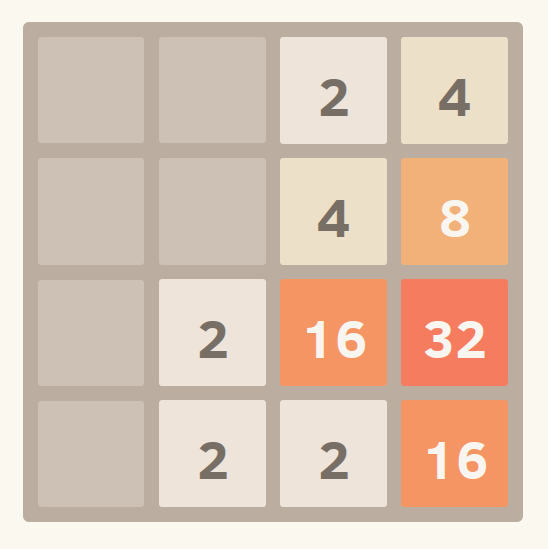
\includegraphics[width=2.0in]{2048_Screenshot}
	\caption{An example game board. This image is obtained from Wikipedia.}
	\label{fig:game_board}
\end{figure}

\subsubsection{Relationship Representation}
Reading Barto's "Reinforcement Learning" book, I have learnt that, to improve my learning, my state vector needs to have information involving interaction between the tiles. In addition to that, I have also decided to use the book's convention where the action dependency will be put in the state instead of the weight vector. This means our Linear Approximation equation can be re-written as:
\begin{equation*}
q_{a} = \phi(a)^{T} w
\end{equation*}
When we play the game, whenever we consider a horizontal move, we always compare the tiles horizontally.  This means the interaction considered will be horizontal. We will represent the interaction by the difference between 2 tiles. Our state vector for move left will then be written as:
\begin{equation*}
\phi(L) = (\mbox{values of all 16 tiles}, \mbox{horizontal differences between each tile of each row})^{T}
\end{equation*}
To distinguish move "L" and "R" the horizontal differences in $\phi(R)$ will have opposite sign to that in $\phi(L)$. $\phi(U)$ and $\phi(D)$ can be calculated with similar method except we will consider vertical differences instead.  

\subsection{Actions}
As explained before, there are 4 available actions for the agent to choose from. They are "Left", "Right", "Up" and "Down". Our agent will choose the action by calculating the q-value of each action. Since there are lots of possible traces in this game, we choose the action using the epsilon-greedy policy to allow exploration by the agent. The epsilon-greedy policy is:

\begin{equation}
\pi(s,a) = \begin{cases} 1-\epsilon+\frac{\epsilon}{|A|}, & a = argmax_{a'}(q(s, a'))\\ \frac{\epsilon}{|A|} & \mbox{otherwise} \end{cases} \
\end{equation}
where $|A|$ is the number of available actions the agent has. In our case, $|A|$ will be most likely to be 4. As mentioned above, there are a huge possibility of traces in this game. To ensure we don't waste time exploring invalid moves, we have decided to restrict our agent to only choose from valid moves. This means if "Left" is not a valid move, we will only have 3 actions available for the agent to choose from and $|A| = 3$ in this case instead assuming the other 3 moves are still valid. 
\\

From multiple sources, I have also seen that instead of using a pure epsilon-greedy policy, people tend to use a decaying epsilon-greedy policy. This allows exploration at the beginning but it decreases the freedom of exploration as we get to the later episodes of the learning process. We have implemented this by a rather naive step-wise decaying scheme.  

\subsection{Reward Schemes}
Multiple reward schemes has been attempted and they both have their merit and drawbacks. We started off with a simple reward scheme where it will reward the value of the greatest value on the board after a move. For example, if after a move we obtain a board state shown in figure \ref{fig:game_board}, we will get 32 points. 
\\

Another reward scheme we have attempted will be the merge-reward scheme, where the agent will be rewarded whenever we merge two tiles into one. The reward will be the value of the new tile. For example, if the initial board is that shown in figure \ref{fig:game_board} and we move right, the two "2"s in the bottom role will merge and give a new tile "4". This will give us 4 points.

\subsection{Learning}
We have mainly used the q-learning equation when updating the weight vector, which is:
% note this uses the align environment
\begin{align}
% \input and \weights in this equation are defined using a macro 
% see the \newcommand lines at the top
\Delta w_a
% & helps neatly align equations over multiple lines 
& = \alpha(R_{t+1} + \gamma \mbox{max}_{a}(S_{t+1} (a), w_{t+1}) - q(S_{t}; w_{t})  \nabla_{w} q(S_{t}; w_{t}))
\\ % line break
& =  \alpha(R_{t+1} + \gamma \mbox{max}_{a}(S_{t+1} (a), w_{t+1}) - q(S_{t}; w_{t})  S_{t}))
\notag % don't give this line an equation number
\end{align}
where we have taken $\alpha = 0.0000001$, $\gamma = 0.9$. 
\\

We used the decaying-epsilon-greedy policy as explained above with $\epsilon=0.1$ initially. Finally, we have decided to play the game with at least 1000 episodes.

